\documentclass{article}
\usepackage[utf8]{inputenc}
\usepackage{graphicx}
\usepackage{amssymb}
\usepackage{placeins}
\usepackage{amsmath}
\usepackage{amsthm}
\usepackage{cite}
\usepackage[citecolor=blue,colorlinks=true,linkcolor=blue]{hyperref}
\usepackage{bm}
\usepackage[margin=1in]{geometry}

\newcommand{\partder}[2]{\dfrac{\partial  #1}{\partial  #2}} % partial der.
\newcommand{\der}[2]{\dfrac{d #1}{d  #2}}

\title{Rotation and Neoclassical Ripple Transport in ITER}
\begin{document}
\maketitle

\begin{abstract}

Neoclassical interactions with non-axisymmetric magnetic fields cause a toroidal torque known as neoclassical toroidal viscosity (NTV). The toroidal symmetry of ITER will be broken by the finite number of toroidal field coils and the presence of perturbing ferromagnetic structures such as test blanket modules (TBMs) and ferritic inserts (FIs). 3D magnetic equilibria are calculated for an ITER steady-state scenario using the Variational Moments Equilibrium Code (VMEC), and neoclassical transport quantities in the presence of these error fields are calculated using the Stellarator Fokker-Planck Iterative Neoclassical Solver (SFINCS). As NTV is a complicated non-linear function of $E_r$, we study its behavior over a plausible range of $E_r$. We estimate the toroidal flow, and hence $E_r$, using a semi-analytic turbulent intrinsic rotation model. The magnitude of NTV torque density at large radii ($r/a \gtrsim$ 0.7) is comparable to the NBI torque density at small radii ($r/a \lesssim$ 0.4), but is opposite in direction and may significantly damp rotation in the edge. The FIs decrease neoclassical transport, while the TBMs have little effect on rotation. 
\end{abstract}

\section{Introduction}

Toroidal rotation is crucial to the experimental control of tokamaks: the magnitude of rotation is known to suppress resistive wall modes \cite{Bondeson1994, Garofalo2002}, while rotation shear can decrease microinstabilities and promote formation of transport barriers \cite{Burrell1997, Terry2000}. As some ITER scenarios will be above the no-wall limit \cite{Liu2004}, it is important to understand the sources and sinks of angular momentum for stabilization of external kink modes. One such sink is the toroidal torque caused by 3D non-resonant error fields. This change in rotation due to the breaking of toroidal symmetry of $B$ has been observed in the Joint European Tokamak (JET) \cite{Lazzaro2002, DeVries2008}, DIII-D \cite{Garofalo2008}, and NSTX \cite{Zhu2006}. 

In addition to the ripple due to the finite number (18) of toroidal field (TF) coils, the magnetic field in ITER will be perturbed by the addition of ferromagnetic components including ferritic inserts (FIs) and test blanket modules (TBMs). TBMs will be installed in three equatorial ports in order to test tritium breeding and extraction of heat from the blanket. The structural material for these modules is ferritic steel and will produce additional error fields in response to the background field. The TBMs will be installed during the H/He phase in order to test their performance in addition to their possible effects on confinement and transport \cite{Chuyanov2010}. It is important to understand their effect on transport during the early phases of ITER, including their influence on angular momentum transport. Experiments at DIII-D including mock-ups of TBMs indicated a reduction in toroidal rotation by as much as 60\% due to magnetic braking \cite{Schaffer2011}. However, neoclassical transport will likely differ in ITER due to its low collisionality and $\rho_*$. FIs are ferritic steel plates that will be installed in each of the toroidal field coil sections in order to mitigate energetic particle loss due to TF ripple \cite{Tobita2003}. As FIs will decrease toroidal field ripple, they may decrease the magnetic braking in ITER. 

In the presence of non-axisymmetric error fields, the bounce-averaged radial particle drifts will not necessarily vanish. Several effects can give rise to non-zero radial current: particles trapped poloidally can experience a net radial drift (banana diffusion), and particles may become trapped in magnetic wells caused by the perturbing field (ripple trapping). For a general electric field, the electron and ion fluxes would not be identical. Ions tend to dominate neoclassical ripple transport, and the resulting particle flux is non-ambipolar. As ambipolarity must be restored for charge conservation, a radial electric field develops to hold the ions back. The radial current caused by outward ion flow induces a $\bm{J} \times \bm{B}$ torque which is typically counter-current, often referred to as neoclassical toroidal viscosity (NTV). Analytic expressions for neoclassical fluxes in several rippled tokamak transport regimes have been derived, making assumptions about the magnitude of the perturbing field and the electric field, magnetic geometry, the collisionality, and the collision operator \cite{Shaing2003, Shaing2008, Shaing2010}. Rather than applying this simplified theory, in this paper a drift kinetic equation is solved using the Stellarator Fokker-Planck Iterative Neoclassical Solver (SFINCS) \cite{Landreman2014} to calculate neoclassical torque and heat flux for an ITER steady-state scenario. The SFINCS code does not exploit any expansions in collisionality, size of perturbing field, or magnitude of the radial electric filed. It also allows for realistic experimental magnetic geometry rather than using simplified flux surface shapes. 
%An additional torque will arise due to the ripple trapping of NBI particles but is predicted to be small \cite{Rosenbluth1996}.  % mention total radial current must vanish here?

In addition to NTV torque, the rotation profile in ITER will be determined by turbulence and neutral beam injection (NBI). 
Because of ITER's high particle energy $E = 1$ MeV for input power $P$ = 33 MW, ITER's neutral beams will provide less momentum than in other tokamaks such as JET, with 125 kV particle energy for similar input power \cite{Ciric2011}, as torque scales as $P/E^{1/2}$. NBI-driven rotation will also be smaller in ITER because of its relatively large moment of inertia, with major radius $R = 6$ m compared to 3 m for JET for comparable densities. 

However, spontaneous rotation may be significant. Turbulence can drive significant flows in the absence of external momentum injection, known as intrinsic or spontaneous rotation, and this effect may be significant in ITER. This can be understood as a redistribution of turbulent momentum to produce large directed flows; in the case of tokamaks this must be in the (approximate) symmetry direction. According to gyrokinetic orderings and inter-machine comparisons by Parra \cite{Parra2012}, intrinsic rotation scales as $\sim \Delta T_i/I_p$, and core rotations may be on the order of 100 km/s in ITER. Rice's scaling based on multi-experiment data \cite{Rice2007} predicts a much larger rotation, $V_{\zeta} \propto \Delta W_p/I_p \sim 700$ km/s, where $W_p$ is the stored plasma energy and $I_p$ is the plasma current. Co-current toroidal rotation appears to be a common feature of H-mode plasmas and has been observed in electron cyclotron heated (ECH)\cite{DeGrassie2007}, ohmic \cite{DeGrassie2007}, and ion cyclotron range of frequencies (ICRF) \cite{Noterdaeme2003} heated plasmas. Gyrokinetic GS2 simulations have also shown that low collisionality tokamaks have an inward radial momentum flux, corresponding to a rotation profile peaked in the core toward the co-current direction \cite{Barnes2013}. In an up-down symmetric tokamak, radial intrinsic angular momentum flux can be shown to vanish to lowest order in $\rho_* = \rho_i/a$ where $a$ is the minor radius, but neoclassical departures from an equilibrium Maxwellian can break this symmetry and cause non-zero rotation in the absence or input momentum \cite{Barnes2013}. This type of symmetry-breaking will be considered in calculating anomalous rotation in section \ref{rotation}. 

In section \ref{steadystate} the ITER steady state scenario considered is discussed. In section \ref{vmec} free boundary magnetohydrodynamic (MHD) equilibrium in the presence of field ripple are presented. Section \ref{rotation} presents estimation of NBI-driven rotation as well as turbulent rotation. This flow velocity is related to $E_r$ in section \ref{Erandv}. These calculations are used to determine neoclassical transport, as NTV torque is a non-linear function of $E_r$. The influence of TF ripple, TBMs, and FIs on neoclassical transport is evaluated, and a radial profile of torque is presented in section \ref{torque}. In section \ref{scaling} the scaling of transport calculated with SFINCS is compared with that predicted by NTV theory, and in section \ref{heatflux} neoclassical heat fluxes in the presence of ripple are presented. In section \ref{mds}, we assess the influence of several radially-local magnetic drift schemes on the transport for this ITER scenario. In section \ref{summary} we summarize the results and conclude.

\section{ITER Steady State Scenario}\label{steadystate}

\FloatBarrier

\begin{figure}[h!]
\centering
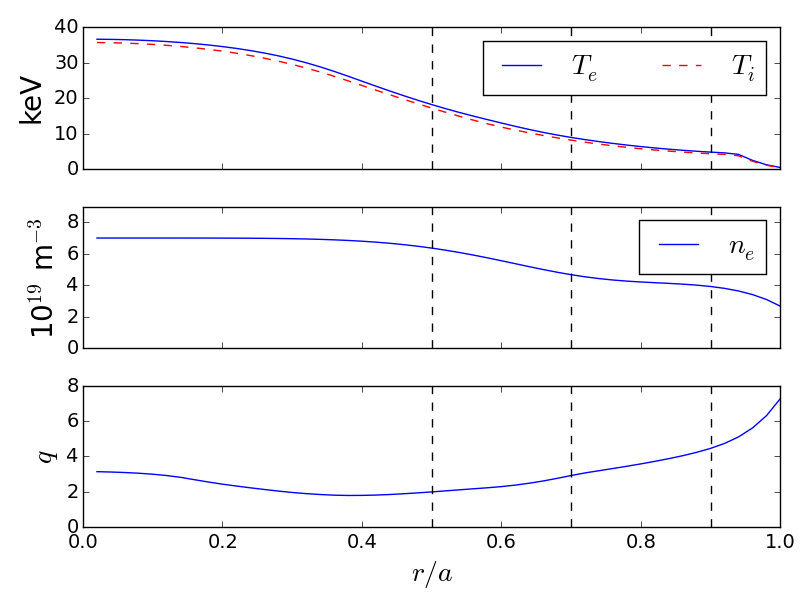
\includegraphics[width=0.7\textwidth]{profiles.png}
\caption{\label{fig:profiles} Radial profiles of temperature, density, and safety factor for the ITER steady state scenario \cite{Poli2014}. Black dashed lines indicate the radial locations that will be considered for neoclassical calculations.}
\end{figure}

We consider an advanced ITER steady state scenario with significant bootstrap current and reversed magnetic shear \cite{Poli2014}. The input power includes 33 MW NBI, 20 MW electron cyclotron (EC), and 20 MW lower hybrid (LH) heating for a fusion gain of $Q = 5$ and toroidal current of 9 MA. The discharge was simulated using the Tokamak Simulation Code (TSC) \cite{Jardin1986} and TRANSP \cite{Hawryluk1980} using a Coppi-Tang \cite{Jardin1993} transport model and EPED1 \cite{Snyder2011} pedestal modeling. The density, temperature, and safety factor $q$ profiles are shown in figure \ref{fig:profiles}. For neoclassical calculations, impurity species are ignored and it is assumed that $n_D = n_T = n_e/2$. Neoclassical transport will be analyzed at the radial locations indicated by dashed horizontal lines ($r/a = 0.5, 0.7, 0.9$). Throughout we will use the radial coordinate $r/a = \sqrt{\Psi_T/\Psi_T^{\text{edge}}}$ where $\Psi_T$ is the toroidal flux and $\Psi_T^{\text{edge}}$ is the toroidal flux at the last surface.

\FloatBarrier

\section{Free Boundary Equilibrium Calculations and Ripple Magnitude} \label{vmec}

The magnetic equilibrium was computed using the density, temperature, and $q$ profiles from TRANSP along with filamentary models of the toroidal field (TF), poloidal field (PF), and center stack (CS) coils and their corresponding currents. The vacuum fields produced by the three TBMs and the FIs have been modeled using FEMAG \cite{Shinohara2009}. The VMEC free-boundary equilibrium \cite{Hirshman1986} is computed for four geometries: (i) including only the toroidal field ripple (ii) including TF ripple, TBMs, and FIs, (iii) TF ripple and FIs, and (iv) axisymmetric geometry.  

We define the magnitude of the magnetic field ripple to be $\delta_B = (B_{max}-B_{min})/(B_{max} + B_{min})$, where the maximum and minimum is evaluated at fixed radius and poloidal angle $\theta$. In figure \ref{fig:ripplecontour}, $\delta_B$ is plotted on the poloidal plane for the three rippled VMEC equilibria. The components of $B$ with torodial mode number $n = \pm 18$ were removed from the case with TBMs and FIs in order to demonstrate the magnitude of the ripple produced by the TBMs alone (bottom right). When only toroidal field ripple is present, significant ripple persists over the entire outboard side, while in the configurations with ferritic inserts the ripple is much more localized in $\theta$. When TBMs are also present the ripple is higher in magnitude (1.4\%) around the outboard midplane, while in the other magnetic configurations $\delta_B \approx$ 1\% near the outboard midplane. For comparison, the TF ripple during standard operations is $0.08\%$ in JET \cite{DeVries2008} and $0.6\%$ in ASDEX Upgrade \cite{Martitsch2016}. 

In figure \ref{fig:toroidalripple}, the magnitude of $B$ is plotted as a function of toroidal angle $\zeta$ at $\theta = 0$ and $\theta = \pi/4$. Away from the midplane ($\theta = \pi/4$) the ferritic inserts greatly decrease the magnitude of the 18$^{\text{th}}$ harmonic of the perturbing field due to the finite number of TF coils. Near the midplane the FIs do not decrease the magnitude of this toroidal ripple as strongly, as the number of steel plates will be higher away from the midplane \cite{Shinohara2009}. The TBMs add an additional perturbation around $\theta = 0$, as the TBM ports will be located about the midplane. 

\FloatBarrier

\begin{figure}[h!]
\centering
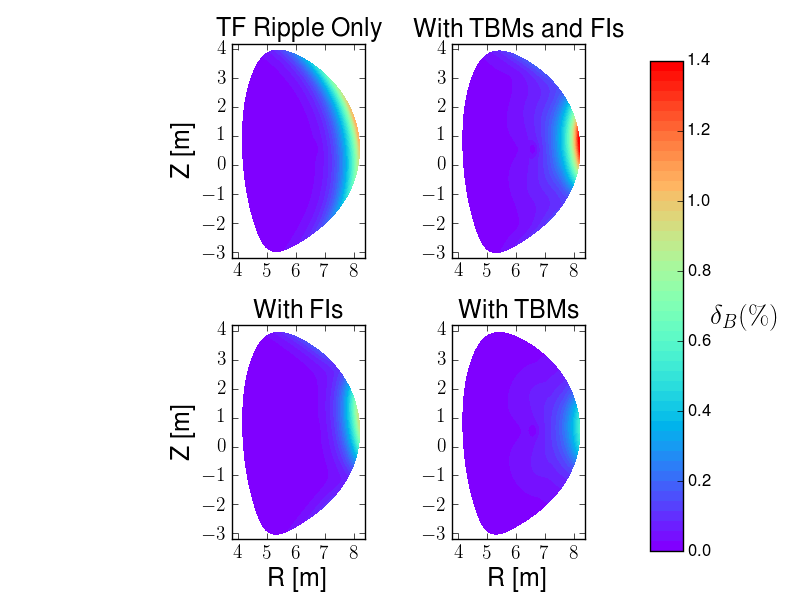
\includegraphics[width=0.7\textwidth]{ripplecontour.png}
\caption{\label{fig:ripplecontour} Magnetic field ripple, $\delta_B = (B_{max}-B_{min})/(B_{max} + B_{min})$, is plotted on the poloidal plane for VMEC free boundary equilibria: (i) including only the toroidal field ripple (top left), (ii) including TF ripple, TBMs, and FIs (top right), (iii) including TF ripple and FIs (bottom left), and (iv) with TBMs only (bottom right). FIs decrease the radial extent of the ripple, while TBMs add an additional ripple near the outboard midplane.}
\end{figure}

\begin{figure}[h!]
\centering
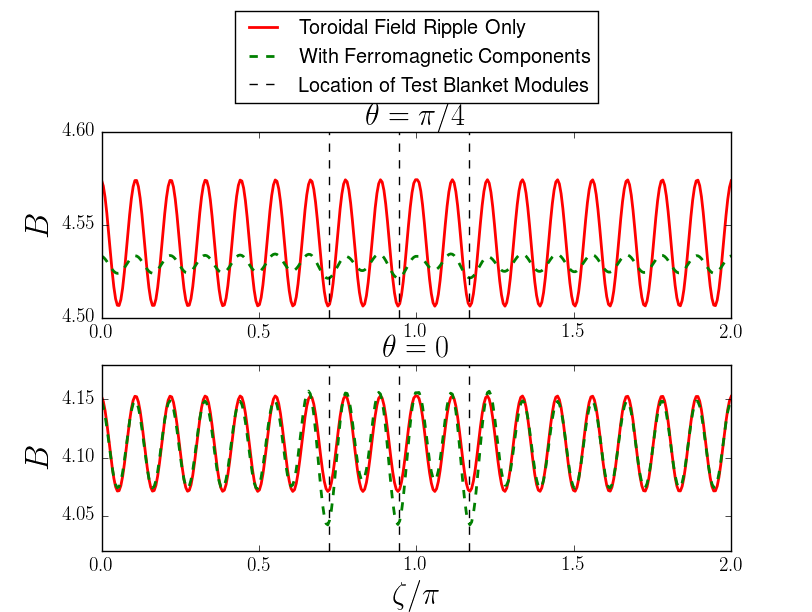
\includegraphics[width=0.7\textwidth]{toroidalripple.png}
\caption{\label{fig:toroidalripple} The magnitude of $B$ as a function of toroidal angle ($\zeta$) at $r/a = 1$, $\theta = 0$ and $\pi/4$. Vertical dashed lines indicate the toroidal locations of the TBM ports. The mitigating effect of the FIs is stronger away from the midplane, where an increased number of steel plates are inserted. The TBMs add an additional ripple near their locations at the $\theta = 0$. }
\end{figure}

\FloatBarrier

\section{Estimating Toroidal Rotation}\label{rotation}

In order to make predictions of the ripple transport in ITER, the radial electric field, $E_r = - \Phi'(r) $, upon which neoclassical transport depends non-linearly, must first be estimated. This is equivalent to predicting the parallel flow velocity, $V_{||}$, which scales monotonically with $E_r$. Throughout the paper, the $||$ subscript will denote the component of a vector in the $\bm{b} = \bm{B}/B$ direction. As we simply wish to determine a plausible value of $E_r$, the difference between $V_{||}$ and $V_{\zeta}$, the toroidal flow, will be unimportant for our estimates. In this calculation of $V_{\zeta}$ the neoclassical torque is ignored: instead $E_r$ is viewed as an input to neoclassical calculations from which the NTV torque can be obtained. 

For this rotation calculation, angular momentum transport due to neutral beams and turbulence will be considered. There will be an additional torque caused by the radial current of orbit-lost alphas \cite{Rosenbluth1996}, but it will be negligible ($\approx 0.006$ Nm/m$^3$). The following time-independent momentum balance equation is considered in determining $V_{\zeta}$,
\begin{gather}
\nabla \cdot \Pi_{\zeta}^{turb}(V_{\zeta}) + \nabla \cdot \Pi_{\zeta}^{NC}(V_{\zeta}) = \tau^{NBI},
\end{gather}
where $\Pi^{turb}_{\zeta}$ and $\Pi^{NC}_{\zeta}$ are the toroidal angular momentum flux densities due to turbulence and neoclassical effects and $\tau^{NBI}$ is the NBI torque density. For this paper the feedback of $\Pi_{\zeta}^{NC}$ on $V_{\zeta}$ will not be calculated. The determination of the change in rotation due to NTV would require iteratively solving this equation for $V_{\zeta}$, as both $\Pi_{\zeta}^{turb}$ and $\Pi_{\zeta}^{NC}$ are functions of $V_{\zeta}$. $\Pi_{\zeta}^{turb}$ consists of a diffusive term as well as a term independent of $V_{\zeta}$ which accounts for turbulent intrinsic rotation. An angular momentum pinch will not be considered for this analysis. 
\begin{gather}
\Pi_{\zeta}^{turb} = -m_i n_i \chi_{\zeta} \langle R \rangle\partder{V_{\zeta}}{r} + \Pi_{int}
\end{gather}
Here $\langle R \rangle$ is the flux-surface averaged major radius and $m_i$ and $n_i$ are the ion mass and density. As it is difficult to model the interactions between external torques and intrinsic rotation, these two effects are considered separately in order to generate two estimates for $V_{\zeta}$. To estimate NBI-drive rotation, TRANSP evolves the rotation profiles by balancing turbulent diffusion (assuming $\chi_{\zeta} = \chi_{i}$) and models of neutral beam torques from NUBEAM. 
\begin{gather}
\tau^{NBI} = -m_i n_i \chi_{i} \langle R \rangle \partder{V_{\zeta}}{r},
\end{gather}
where $\tau^{NBI}$ is the total beam torque density calculated by NUBEAM including collisional, $\bm{J} \times \bm{B}$, thermalization, and recombination torques.

For the second estimate of toroidal rotation a semi-analytic intrinsic rotation model is used \cite{Hillesheim2015}:
\begin{gather}
V_{\zeta}(r) = - \langle R \rangle \int_{r}^a \frac{v_{ti} \rho_{*,\theta}} {2 P_r L_T^2} \widetilde{\Pi} (\nu_*) \, d r',
\end{gather} \label{eq:Hillesheim}
where $v_{ti}$ is the ion thermal velocity, $\rho_{*,\theta} = v_{ti} m_i/(e B_{\theta} \langle R \rangle) $, the Prandtl number $P_r = \chi_{\zeta}/\chi_i$ is taken to be 0.7, $\nu_* = q R v_{ti}/(\nu_{ii} \epsilon^{3/2})$ is the normalized collision frequency, and $L_T = - \left( \partial \ln T/ \partial r \right)^{-1}$ is the temperature gradient scale length. Equation \ref{eq:Hillesheim} is obtained from assuming that $\Pi_{int}$ balances turbulent momentum diffusion in steady state, $\Pi_{int} = m_i n_i \chi_{\zeta} \langle R \rangle \partial V_{\zeta}/\partial r$. This model considers the intrinsic torque driven by the neoclassical diamagnetic flows, such that $V_{\zeta} \sim \rho_{*,\theta} v_{ti}$ and $(V_{\zeta}/\langle R \rangle) \Pi_{int}/Q \sim \rho_{*, \theta}$. It is also assumed that $V_{\zeta} = 0$ at the wall. %Provide justification for these assumptions?? 
$\widetilde{\Pi} (\nu_*)$ is an order unity function which characterizes the collisionality dependence of rotation reversals, determined from gyrokinetic turbulence simulations \cite{Barnes2013}. Because of the ITER's low collisionality, we do not expect a rotation reversal, which is correlated with transitioning between the banana and plateau regimes. Equation \ref{eq:Hillesheim} was integrated using profiles for the ITER steady state scenario. 

The results of these two rotation models are shown in figure \ref{fig:rotation_estimate}. NBI torque contributes to significant rotation at $r/a \lesssim 0.4$, where the torque density also peaks (see figure \ref{fig:alltorque}).  At the radii that will be considered for neoclassical calculations (indicated by dashed vertical lines), intrinsic turbulent rotation may dominate over that due to NBI. Therefore, for the purposes of estimating $E_r$ the intrinsic rotation calculation of $V_{\zeta}$ will be used. $V_{\zeta}$ from this model is comparable to that predicted from theoretical scaling arguments \cite{Parra2012}. However, it should be noted that $V_{\zeta}$ shown in \ref{fig:rotation_estimate} is an estimate based on scaling arguments, as much uncertainty is inherent in predicting turbulent rotation. We simply use this to estimate the value of $E_r$ in ITER which determines the neoclassical transport regime. 

\FloatBarrier

\begin{figure}[h!]
\centering
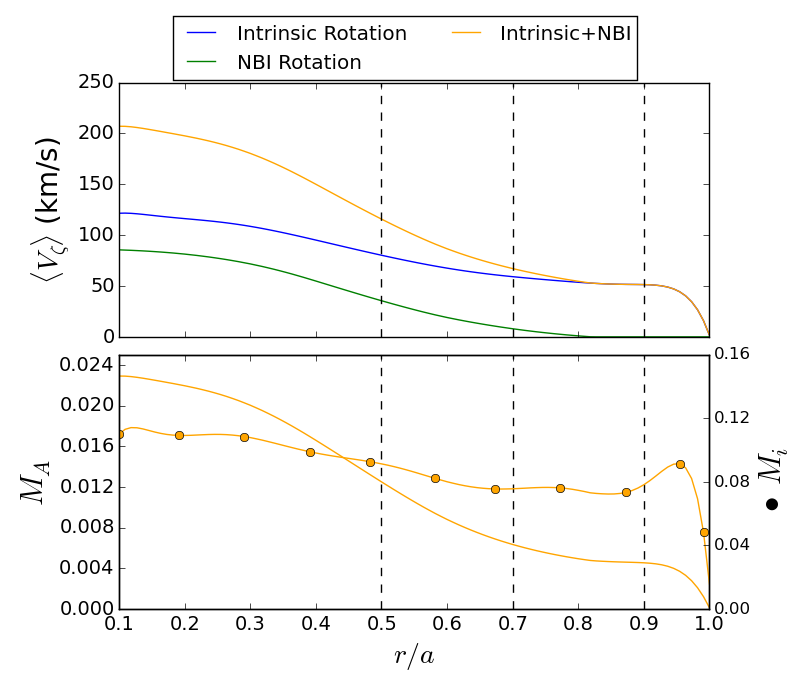
\includegraphics[width=0.7\textwidth]{rotationestimate.png}
\caption{\label{fig:rotation_estimate} Toroidal rotation $V_{\zeta}$ due to turbulence and NBI (top) is shown along with  corresponding Alfv\`{e}n Mach number (bottom, solid), and sonic Mach number (bottom, bulleted). The intrinsic rotation calculation uses a semi-analytic model of turbulent momentum redistribution \cite{Hillesheim2015}. The NBI rotation is calculated from turbulent diffusion of NBI torque using NUBEAM and TRANSP \cite{Poli2014}. Dashed vertical lines indicate the radial positions where SFINCS calculations are performed. }
\end{figure}

For stabilization of the resistive wall mode (RWM) in ITER, it has been estimated that a critical central rotation frequency of $\gtrsim5\%$ of the Alfv\`{e}n frequency, $\omega_A = B/(\langle R\rangle\sqrt{\mu_0 \rho_i})$, must be achieved given a peaked rotation profile. Additionally, the TBM are known to increase the critical rotation frequency as they have a much shorter $L/R$ time scale than the wall \cite{Liu2004}. Given the central rotation frequency $\omega_0/\omega_A \sim 2\%$ in figure \ref{fig:rotation_estimate}, it may be difficult to suppress the RWM in ITER with rotation alone. As this calculation does not take into account magnetic braking, $\omega_0/\omega_A$ will most likely be smaller than what is shown. 

\FloatBarrier

\section{Relationship Between $E_r$ and $V_{||}$}\label{Erandv}

Equipped with a profile of $V_{\zeta}$, neoclassical calculations of $V_{||}$ are made in order to determine the radial electric field. The parallel flow velocity for species $s$ is calculated from moments of the neoclassical distribution function,
\begin{gather}
V^s_{||} = \left(\frac{1}{n_s}\right
) \int d^3 v \, v_{||} f_s,
\end{gather}
which we calculate with the Stellarator Fokker-Planck Iterative Neoclassical Conservative Solver (SFINCS) \cite{Landreman2014} code.
SFINCS is used to solve a radially-local drift kinetic equation for the gyro-averaged distribution function, $f_{a1}$, on a single flux surface including coupling between species. 
\begin{gather}
( v_{||} \bm{b} + \bm{v}_E + \bm{v}_{ma}) \cdot (\nabla f_{a1})  - C(f_{a1}) = - \bm{v}_{ma} \cdot \nabla \psi \left( \partder{f_{a0}}{\psi} \right) + \frac{Z_a e v_{||} B \langle E_{||} B \rangle}{T_a \langle B^2 \rangle } f_{a0}.
\end{gather} \label{kineticequation}
\hspace{-1mm}
Here $a$ indicates species, $f_{a0}$ is an equilibrium Maxwellian, $ \langle ... \rangle$ denotes a flux surface average, $\psi = \Phi_T/2\pi$, and $C$ is a linearized Fokker-Planck collision operator. The $\bm{E} \times \bm{B}$ drift is 
\begin{gather}
\bm{v}_E = \frac{1}{B^2} \bm{B} \times \nabla \Phi
\end{gather} 
and the radial magnetic drift is
\begin{gather}
\bm{v}_{ma} \cdot \nabla \psi = \frac{m_a }{2Z_a e B^2} \left(v_{||}^2 + \frac{v_{\perp}^2}{2} \right) \bm{b} \times \nabla B \cdot \nabla \psi,
\end{gather} \label{magneticdrift}
where $v_{||}$ and $v_{\perp}$ are the components of the velocity coordinate parallel and perpendicular to $\bm{B}$, respectively. Transport quantities have been calculated using the steady state scenario ion and electron profiles and VMEC geometry. The $E_{||}$ term is negligible for this non-inductive scenario with loop voltage $ \approx 10^{-4}$ V. For the calculations presented in this section and in section \ref{heatflux} the $\bm{v}_{ma} \cdot \nabla f_{a1}$ term is dropped. The effect of keeping this term is shown to be small in section \ref{mds}.

The relationship between $E_r$ and $V_{||}$ for electrons and ions at $r/a = 0.9$ is shown in figure \ref{fig:Er_flow}. Note that only one curve is shown for each species as the addition of ripple fields did not change the dependence of $V_{||}$ on $E_r$ significantly ($\leq 5 \%$). While radial transport of heat and particles changes significantly in the presence of small ripple fields, the parallel flow is much less sensitive to the perturbing field. Only the component of $f$ that is odd in $v_{||}$ will contribute to $V_{||}$, while only the component even in $v_{||}$ will contribute to $\Gamma_{\psi}$. It can be shown (see appendix \ref{parallelflow}) that the component of $f_1$ that contributes to $V_{||}$ is of higher order in $\nu_* = \nu_{ii} Rq/(\epsilon^{3/2} v_{ti}) \ll 1 $, where $\epsilon$ is the inverse aspect ration, than the component that contributes to $\Gamma_{\psi}$. 

\begin{figure}[h!]
\centering
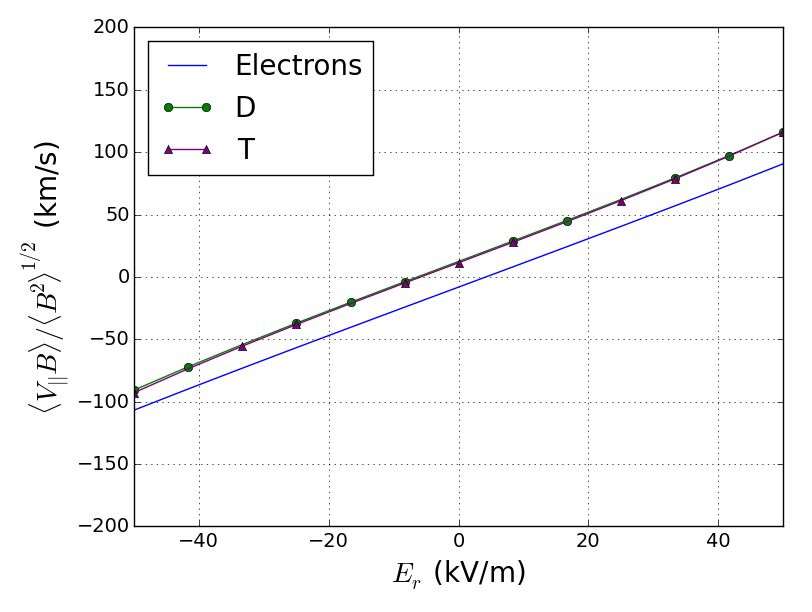
\includegraphics[width=.7\textwidth]{Er_flow.png}
\caption{\label{fig:Er_flow} SFINCS calculation of the parallel flow $V_{||}$ at $r/a = 0.9$ for ions and electrons. Addition of ripple does not change tokamak neoclassical relationship between $E_r$ and $V_{||}$ by a discernable amount on this scale although the radial particle fluxes, $\Gamma_{\psi}$, are sensitive to perturbing field.}
\end{figure}

\FloatBarrier

\section{Torque Calculation}\label{torque}

The NTV torque density, $\tau^{NTV}$, is calculated from radial particle fluxes, $\Gamma_{\psi}$, using the flux-friction relation,
\begin{gather}
\tau^{NTV} = - B^{\theta} \sum_a n_a q_a \Gamma_{\psi, a},
\end{gather}
where $B^{\theta} = \bm{B} \cdot \nabla \theta$ and the summation is performed over species. The calculation of $\tau^{NTV}$ for three geometries at $r/a = 0.9$ is shown in figure \ref{fig:Torque_ErandV}. The axisymmetric geometry does not contribute to NTV torque, as expected. Overall, the magnitude of the torque density with only TF ripple is larger than that with the addition of both the FIs and the TBMs.  In figure \ref{fig:Torque_ErandV} we show that the TBMs alone do not provide significant radial current, so the decrease in torque magnitude with FIs and TBMs can be attributed to the decrease in ripple with the ferritic inserts. The dashed vertical line indicates the value of $V_{||}$ and $E_r$ predicted from the intrinsic rotation model. At this radius for the TF only case, $\tau^{NTV} = -0.058$ Nm/m$^3$ while for the case with TBMs and FIs it is -0.012 Nm/m$^3$. The circle indicates the offset rotation at the ambipolar $E_r$. If no other angular momentum source were present in the system, the NTV torque would drive the plasma to rotate at this velocity. Although the $\tau^{NTV}$ varies significantly between the two geometries they predict similar offset rotation velocities: $V_{\zeta}$ = -10 km/s with TF ripple only and -6 km/s with TBMs and FIs. Note that for $E_r$ greater than this ambipolar value, $\tau^{NTV}$ is counter-current while neutral beams and turbulence drive rotation in the co-current direction, so $\tau^{NTV}$ is a damping torque.

The NTV torque due to TF ripple only is higher in magnitude than the total beam torque while that with TBMs and FIs is of similar magnitude to the beam torque density (see figure \ref{fig:alltorque}). $\tau^{NTV}$ may also compete with the turbulent torque. If $\Pi_{int} \sim \rho_{*, \theta} Q\, \widetilde{\Pi}/(V_{\zeta}/\langle R \rangle)$, the magnitude of the torque density due to turbulence (-$\nabla \cdot \Pi_{int}$) is $\sim 0.05$ Nm/m$^3$. Therefore, NTV torque may be key in determining the edge rotation in ITER.

\FloatBarrier

\begin{figure}[h!]
\centering
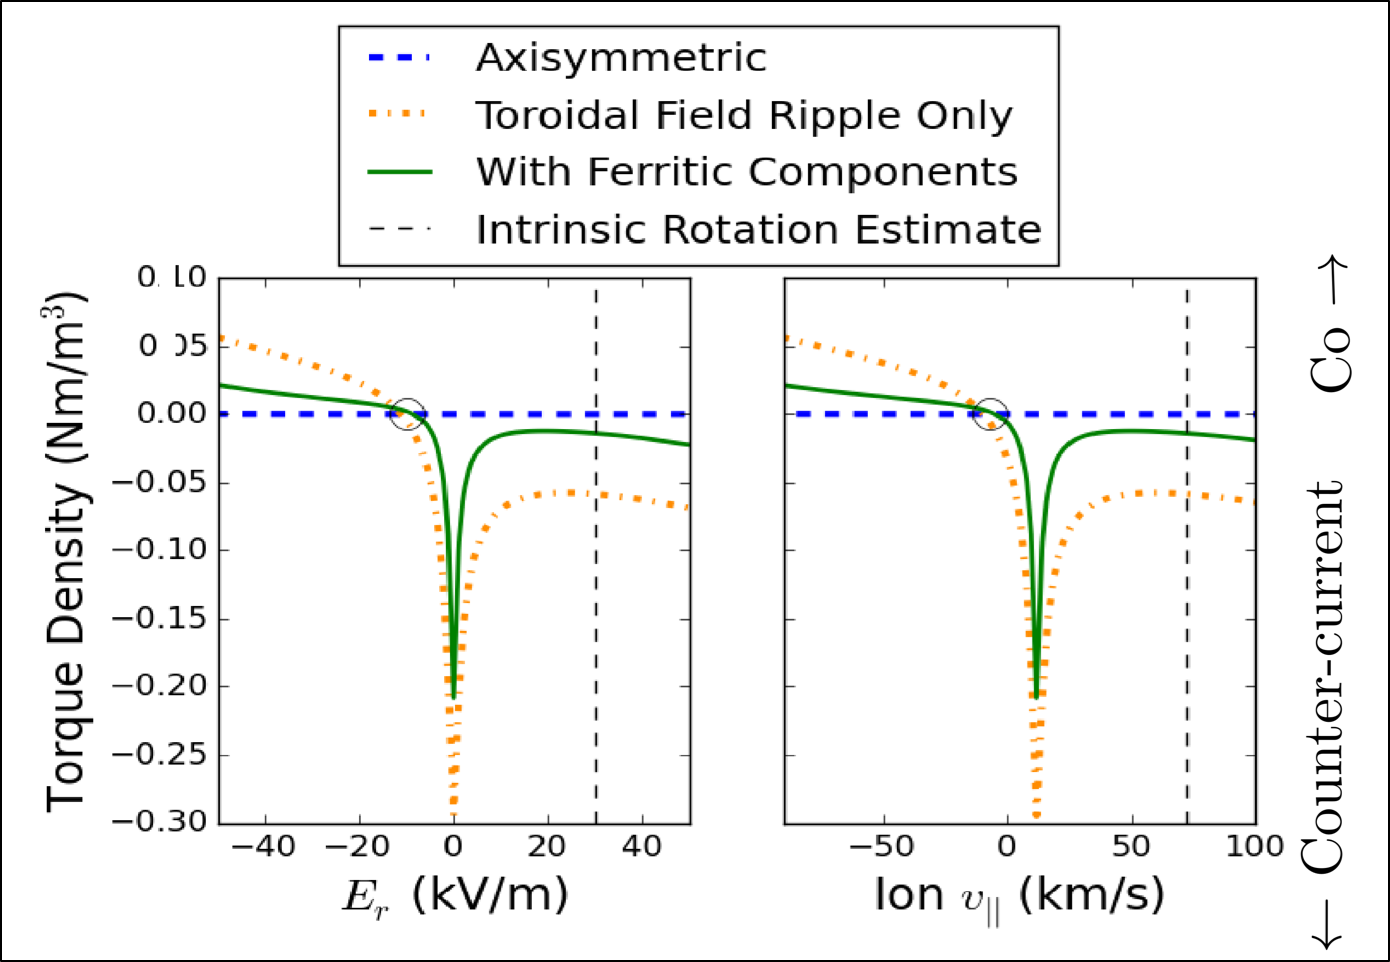
\includegraphics[width=0.7\textwidth]{Torque_ErandV.png}
\caption{\label{fig:Torque_ErandV} SFINCS calculation of NTV torque density as a function of $E_r$ and $V_{||}$ at $r/a = 0.9$ is shown for 3 VMEC geometries: (i) axisymmettic (blue dashed), (ii) with TF ripple only (orange dash-dot), and (iii) TF ripple with FIs and TBMs (green solid). The vertical dashed line indicates the estimate of $E_r$ and $V_{||}$ based on the intrinsic rotation model. The circle denotes the offset rotation at $V_{||} \sim -10$ km/s. The magnitude of $\tau^{NTV}$ at this radius is comparable or greater to the NBI and turbulent torques but is opposite in direction (see figure \ref{fig:alltorque}). }
\end{figure}

In order to decouple the influence of the FI ripple and the TBM ripple, the torque density is calculated at $r/a = 0.9$ for geometries including (i) TF ripple with FIs and TBMs, (ii) TF ripple with FIs, and (iii) only TBMs, shown in figure \ref{fig:Torque_comparingTBMandFI}. The ripple due to the TBMs drives much less $\tau^{NTV}$ than the TF ripple with ferritic inserts does.  While the FIs decrease the magnitude of the $n = 18$ component of $B$, the TBM contributes to low mode numbers (mostly $n = 1$). In the $\sqrt{\nu}$ regime ion transport scales as $\Gamma_{\psi} \sim \sqrt{n}$ and in the $1/\nu$ regime $\Gamma_{\psi} \sim n^2$ \cite{Shaing2010}, so it is reasonable to expect that the higher harmonic ripple of the FIs would drive a larger $\tau^{NTV}$. Moreover, when transport is dominated by the $\bm{E} \times \bm{B}$ precession frequency ($\nu_{\text{eff}}/\omega_E \ll 1$), if the poloidal extent of the ripple $\Delta \theta$ is decreased, the characteristic time scale for detrapping $\Delta t \sim \Delta \theta/ \omega_E$ will decrease. If diffusion scales as $D \sim f_t \Delta x^2/\Delta t$, reducing the poloidal extent of ripple will decrease transport. 

\begin{figure}[h!]
\centering
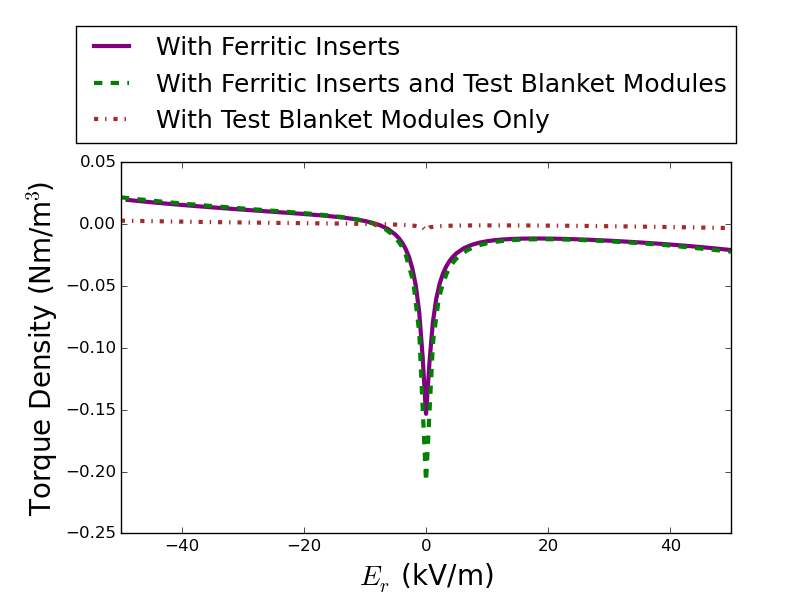
\includegraphics[width=0.7\textwidth]{Torque_comparingTBMandFI.png}
\caption{\label{fig:Torque_comparingTBMandFI} The NTV torque density at $r/a = 0.9$ for three magnetic geometries: (i) with FIs (purple solid), (ii) with TBMs (brown dash dot), (iii) and with FIs and TBMs (green dashed). The TBMs alone do not contribute significantly to neoclassical transport. }
\end{figure}

In figure \ref{fig:Torque_radiusscaling}, the SFINCS calculation of $\tau^{NTV}$ with TF ripple only is shown at $r/a$ = 0.5, 0.7, and 0.9. For these three radii the maximum $\delta_B = 0.26\%$, 0.51\%, and 0.82\% respectively. It is reasonable to expect that the magnitude of transport will decrease with decreasing ripple, as $\Gamma_{\psi} \sim (\delta_B)^2$ in the $1/\nu$ and $\sqrt{\nu}$ regimes and $\sim (\delta_B)$ in the $\nu$ regime \cite{Shaing2010}.  Moreover, the poloidal extent of the ripple decreases with decreasing radius, so particles spend less time in the rippled region and transport should decrease. On the other hand, transport in the $\sqrt{\nu}$ regime scales with $T_i$: $\Gamma_{\sqrt{\nu}} \sim v_{ti}^4 \sqrt{\nu_{ii}} \sim T_i^{5/4}$. This $\sqrt{\nu}$ regime applies to the region outside the thin `valley' near $E_r$ = 0, where $\omega_E > \nu_{ii}/\epsilon$ ($\omega_E = \frac{E_r}{B}$). The combined effect of decreased ripple and increased temperature with decreasing radius leads to comparable torques with decreasing radius in this region. However, the scaling with $T_i$ is even stronger in the $1/\nu$ regime where this `valley' occurs, as $\Gamma_{1/\nu} \sim v_{ti}^4/\nu_{ii} \sim T^{7/2}$. Indeed, we find that the magnitude of $\tau_{NTV}$ at $E_r = 0$ increases with decreasing radius. 

\begin{figure}[h!]
\centering
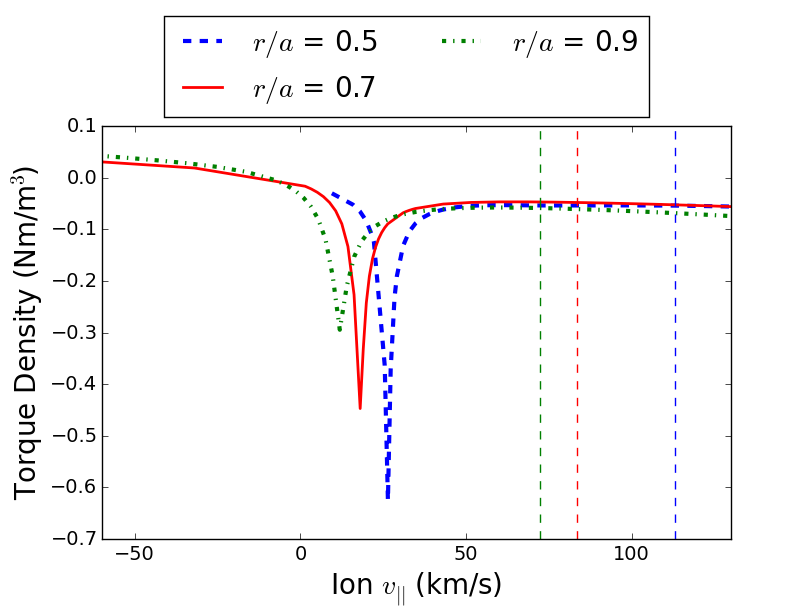
\includegraphics[width=0.7\textwidth]
{Torque_radiusscaling.png}
\caption{\label{fig:Torque_radiusscaling} SFINCS calculation of NTV torque density ($\tau^{NTV}$) as a function of ion $V_{||}$ for VMEC geometry with TF ripple only at $r/a$ = 0.5 (blue solid), 0.7 (red dashed), and 0.9 (green dash-dot). Although the field ripple decreases with radius ($\delta_B = 0.82\%$ at $r/a = 0.9$, $\delta_B = 0.51\%$ at $r/a = 0.7$, $\delta_B = 0.26\%$ at $r/a = 0.5$), transport in the $1/\nu$ `valley' increases with decreasing radius because of strong scaling of neoclassical transport with temperature. }
\end{figure}

In figure \ref{fig:alltorque}, we compare the magnitude of $\tau^{NTV}$ with $\tau^{NBI}$ and the turbulent momentum source causing intrinsic rotation, $\tau^{int} = -\nabla \cdot \Pi_{int}$. For the $\tau^{NTV}$ profile, the intrinsic rotation model is used for determining $E_r$ at each radius. $\tau^{NBI}$ is determined from NUBEAM calculations \cite{Poli2014}. $\tau^{int}$ is estimated using $\Pi_{int} \sim \rho_{\theta}/L_T \widetilde{\Pi}(\nu_*) Q \langle R \rangle/v_{ti} \sim \frac{m}{eB_{\theta}r} \widetilde{\Pi}(\nu_*) Q \langle R \rangle$ and $\tau^{int} \sim -\Pi_{int}/r$. $Q$ is obtained from the fusion product source profile computed by TRANSP. Note that in the pedestal, this model of turbulent torque is large as $\tau^{turb} \sim 1/L_T$. 

Near the edge ($0.5 \lesssim r/a \lesssim 0.9$), NTV torque may dominate the rotation profile and will likely significantly damp rotation, decreasing MHD stability. However, the resulting rotation profile may be sheared because of the significant counter-current source at the edge and co-current NBI source in the core. This may provide a rotation shear as high as $\Delta V_{\zeta}/ \Delta r \approx 0.8 (v_{ti}/R)$ and may large enough to suppress micorturbulence and decease turbulent transport \cite{Hahm1994}. 

\begin{figure}[h!]
\centering
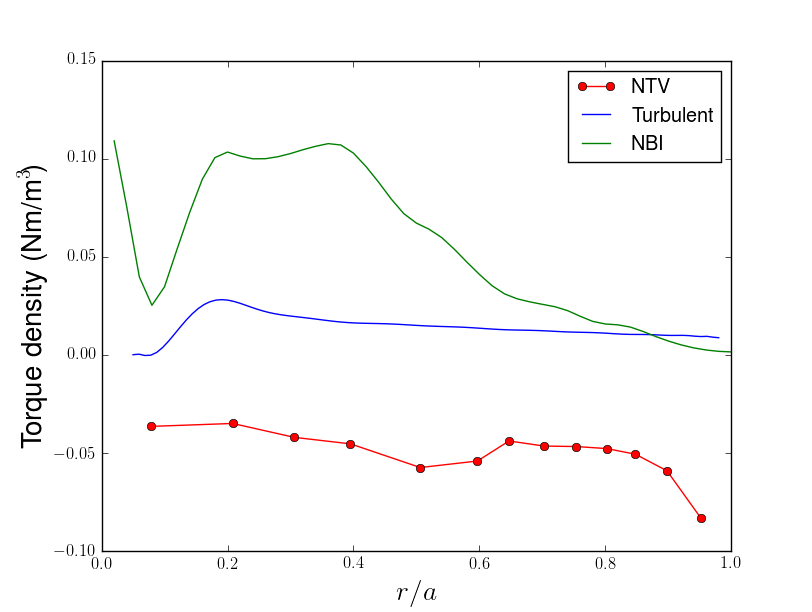
\includegraphics[width=0.7\textwidth]{AllTorquePlot.png}
\caption{Torque density profiles of NTV torque density ($\tau^{NTV}$) calculated with SFINCS, NBI torque density calculated from NUBEAM ($\tau^{NBI}$), and estimate of turbulent intrinsic rotation momentum source ($\tau^{turb}$). $\tau^{NTV}$ is calculated using SFINCS at $E_r$ determined by intrinsic rotation model described in section \ref{rotation}. Turbulent torque is estimated using $\tau^{turb} \sim -\Pi_{int}/a$ where $\Pi_{int} \sim \rho_{*, \theta} \widetilde{\Pi}(\nu_*) Q \langle R \rangle/v_{ti}$.}
\end{figure}\label{fig:alltorque}

\FloatBarrier

\section{Scaling with Ripple Magnitude}\label{scaling}
The scaling of NTV transport with the magnitude of $\delta_B$ shows some agreement with that predicted by Shaing \cite{Shaing2008}. In figure \ref{fig:scalescan}, the NTV torque density calculated by SFINCS is shown as a function of the magnitude of the ripple, $\delta_B$, for TF only geometry. The additional ferromagnetic ripple is not included, while the $n= \pm18$ component of $\bm{B}$ is rescaled. $\tau^{NTV}$ is calculated at $r/a = 0.9$ with $E_r = 30$ kV/m, corresponding to the intrinsic rotation estimate. The color-shaded background indicates the approximate regions of applicability of the $\sqrt{\nu}$ and $\nu$ regimes. The $1/\nu$ regime does not apply at this $E_r$, as $\omega_E \gg \nu/\epsilon$, where $\omega_E = \frac{E_r}{B}$. $E_r$ is also large enough that the resonance between $v_{E}$ and $v_{m}$ cannot occur, so the superbanana plateau and superbanana regimes are avoided. 

In the collisional boundary layer, neoclassical fluxes scale as $\sqrt{\nu}$. This regime becomes relevant when the poloidal $\bm{E} \times \bm{B}$ precession frequency is larger than the effective collision frequency of detrapping banana particles, $\nu/\epsilon < \omega_E$, and the ripple magnitude is not large enough for collisionless detrapping to take effect, $\delta_B < \left(  \epsilon \nu/\omega_E \right)^{1/2}$ \cite{Shaing2008}. 
In the collisionless trapping-retrapping regime, neoclassical fluxes scale with $\nu$. This regime becomes relevant when $\delta_B > \left(  \epsilon \nu/\omega_E \right)^{1/2}$, i.e. the perturbing field becomes large enough that poloidally trapped particles can become detrapped and retrapped by the ripple \cite{Shaing2010}. In the $\sqrt{\nu}$ regime $\tau^{NTV} \sim \delta_B^2$ and in the $\nu$ regime $\sim \delta_B$. For $\delta_B$ smaller than $\delta_B^* = 0.82\%$, the actual value of ripple at $r/a=0.9$ for ITER geometry, the scaling of $\tau^{NTV}$ with $\delta_B$ is slightly shallower than what is predicted. 
As $\delta_B$ nears the boundary between the $\sqrt{\nu}$ and $\nu$ regimes in figure \ref{fig:scalescan}, the scaling of $\tau^{NTV}$ with $\delta_B$ becomes even less stiff and shows some agreement within the $\sqrt{\nu}$ regime. When $\delta_B \sim \epsilon$, the poloidal field variation no longer becomes the dominant perturbation, so $\delta_B \sim \epsilon$ have not been included. The departure of numerical results from predicted scaling can be attributed to the analytic models which uses a bounce-averaged kinetic equation and assumes large aspect ratio. 

\begin{figure}[h!]
\centering
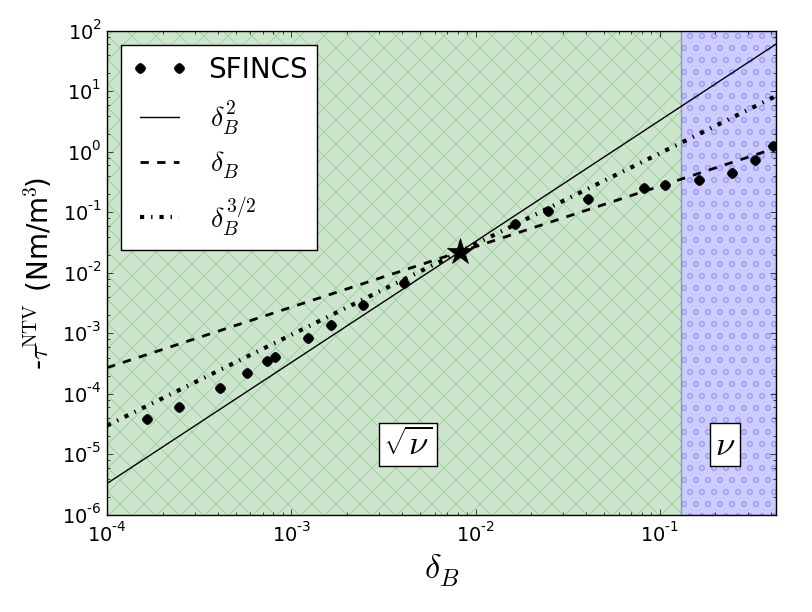
\includegraphics[width=0.7\textwidth]
{scalescan.png}
\caption{\label{fig:scalescan} SFINCS calculations of NTV torque density as a function of $\delta_B$ at $r/a = 0.9$. A single value of $E_r = 30$ kV/m is used corresponding to the intrinsic rotation estimate. Color-shaded area indicates the approximate regions of applicability for rippled tokamak regimes described by Shaing \cite{Shaing2010, Shaing2008}: the $\sqrt{\nu}$ regime where transport scales as $\sim \delta_B^2$ and the $\nu$ regime where $\sim \delta_B$. }
\end{figure} 

\FloatBarrier

\section{Heat Flux Calculation}\label{heatflux}
The breaking of toroidal symmetry drives an additional neoclassical heat flux as well as driving non-ambipolar particle fluxes. In figure \ref{fig:HeatFlux}, the SFINCS calculation of heat flux is shown for three magnetic geometries: (i) axisymmetric (blue solid), (ii) with TF ripple only (green dashed), and (iii) TF ripple with TBMs and FIs (red dash-dot). In the presence of TF ripple, the ripple drives an additional heat flux that is comparable to the axisymmetric heat flux. However, with the addition of the FIs the heat flux is reduced to the magnitude of the axisymmetric value, except near $E_r = 0$ where $1/\nu$ transport dominates. 

While the radial ripple-drive particle fluxes will significantly alter the ITER angular momentum transport, the neoclassical heat fluxes are insignificant in comparison to the turbulent heat flux. Note that at this radius the anomalous heat transport, estimated from the fusion product source profile calculated by TRANSP, amount to $\approx 0.3$ MW/m$^2$, If ITER ripple were scaled up to $\delta_B \gtrsim 30\%$, the neoclassical ripple heat transport would be comparable to the anomalous transport.

\begin{figure}[h!]
\centering
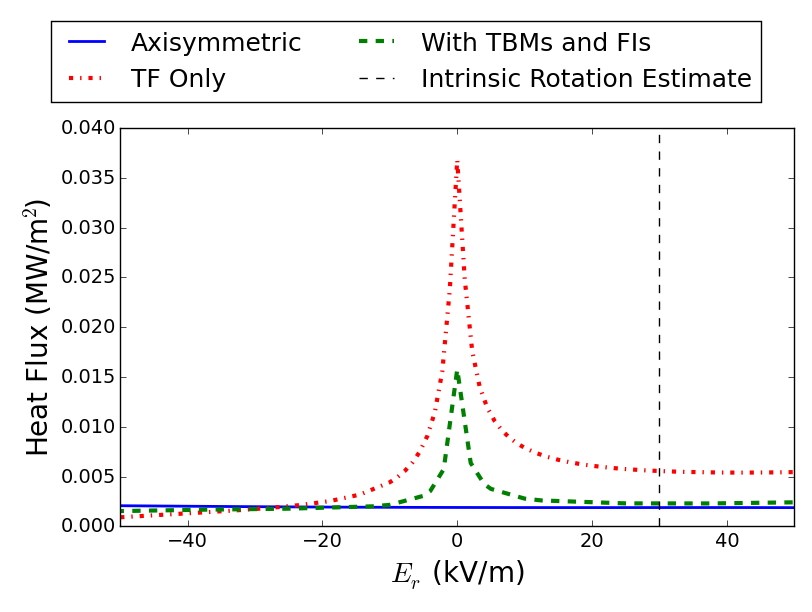
\includegraphics[width=0.7\textwidth]
{HeatFlux.png}
\caption{\label{fig:HeatFlux} SFINCS calculation of neoclassical heat flux at $r/a = 0.9$ for three magnetic geometries: (i) axisymmetric (blue solid), (ii) with TF ripple only (green dashed), and (iii) TF ripple with TBMs and FIs (red dash-dot). The vertical dashed line corresponds to the intrinsic rotation $E_r$ at this radius. These heat fluxes are much smaller than the anomalous heat transport is likely to be, $\approx 0.3$ MW/m$^2$,}
\end{figure}

\FloatBarrier

\section{Radially Local Approximation of Magnetic Drifts}\label{mds}
Although $(\bm{v}_E + \bm{v}_m) \cdot \nabla f_1$ is formally of lower order than the other terms in eq. \ref{kineticequation}, it has been found to be important when $\rho_* \sim \nu_*$ and has been included in other calculations of 3D neoclassical transport. In the SFINCS calculations shown above the $\bm{v}_m \cdot \nabla f_1$ term has not been included. As SFINCS does not maintain radial coupling of $f_1$, there are several radially-local models of toroidal and poloidal $\bm{v}_m$ that can be applied.  The Kasilov form (eq. 67 in \cite{Kasilov2014}) ignores the toroidally varying components of $\bm{B}$ and the radial variation of $q$. The Martitsch form (eq. 16 in \cite{Martitsch2016}) is the same as the Kasilov form but maintains magnetic shear dependence. This non-local effect has been shown to be important in some NTV transport regimes \cite{Martitsch2016}. The Sugama form is obtained by subtracting off the radial component of $\bm{v}_m$ and multiplying by a factor which ensures that $\bm{v}_m (\mu = 0)  = 0$ in order to remove sources/sinks in velocity space. Each of these magnetic drift schemes are independent of the choice of Boozer angle. 

An $E_r$ scan at $r/a = 0.9$ is shown in figure \ref{driftschemes}. When $\bm{v}_m \cdot \nabla f_1$ is added to the kinetic equation, the $1/\nu$ valley is shifted toward a slightly negative $E_r$, corresponding to the region where $\bm{v}_E + \bm{v}_M = 0$. However, the addition of $v_m \cdot \nabla f_1$ has a negligible effect on transport overall, and choice of magnetic drift scheme would not dramatically change the results in previous sections.  

\begin{figure}[h!]
\centering
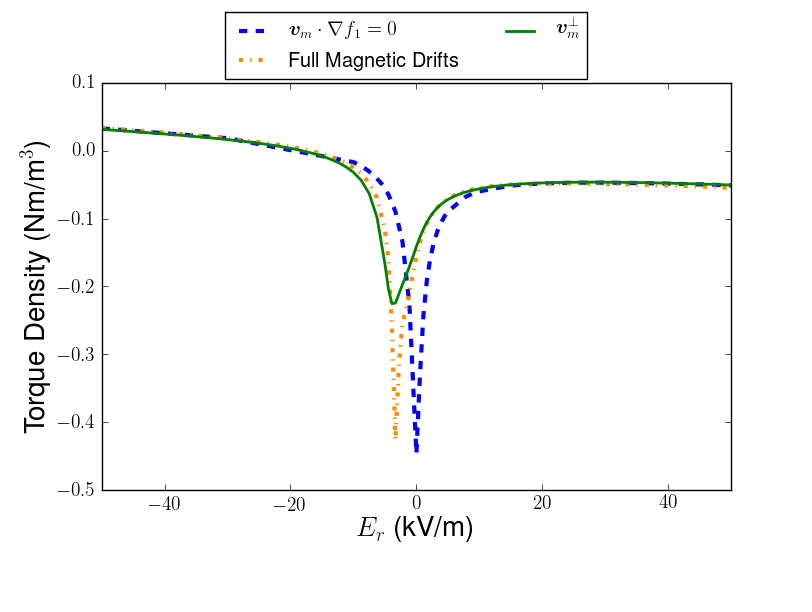
\includegraphics[width=0.7\textwidth]{mdscomparison.png}
\caption{Comparison of magnetic drift models at $r/a = 0.9$. NTV torque density is calculated for the ITER steady state scenario as a function of $E_r$. The addition of $\bm{v}_m \cdot \nabla f_1$ in the kinetic equation solved by SFINCS has little effect on the neoclassical transport at this radius. }
\end{figure}\label{driftschemes}

\FloatBarrier

\section{Summary}\label{summary}

We calculate neoclassical transport in the presence of 3D magnetic fields, including toroidal field ripple and ferromagnetic components, for an ITER steady state scenario. We use an intrinsic turbulent rotation model described in section \ref{rotation} to estimate $E_r$ for neoclassical calculations. We find that even without $\tau^{NTV}$, toroidal rotation will be $\lesssim 2\% M_A$, which is likely not large enough to suppress resistive wall modes \cite{Liu2004}. We use VMEC free boundary equilibria in the presence of ripple fields to calculate neoclassical particle and heat fluxes using the drift-kinetic solver, SFINCS. At large radii $r/a \gtrsim 0.7$, $\tau^{NTV}$ is comparable to $\tau^{NBI}_{\zeta}$ in magnitude but opposite in sign, which may result in flow damping at the edge and a decrease in MHD stability. However, the torque profile may also produce a significant rotation shear which could suppress turbulent transport. While the addition of FIs significantly reduces the transport ($\approx 80\%$ reduction at $r/a = 0.9$), the TBMs themselves produce very little NTV torque. Further analysis is needed to quantify how the addition of $\tau^{NTV}$ will change the rotation profile in ITER. 

\section{Appendix A} \label{parallelflow}
In this appendix we will show that the contribution to $V_{||}$ from $f_1$ is much smaller than the contribution to $\Gamma_{\psi}$. As $V_{||}$ is an odd moment of $v_{||}$,
\begin{gather}
V_{||} = \left(\frac{1}{n_s}\right) \int d^3 v \, v_{||} f,
\end{gather}
only the component of $f_1$ that is odd in $v_{||}$ will contribute. Similarly, only the component of $f_1$ that is even in $v_{||}$ will contribute to $\Gamma_{\psi}$ as it is an even moment of $v_{||}$,
\begin{gather}
\Gamma_{\psi} = \left \langle \int d^3v (\bm{v}_m \cdot \nabla \psi) f \right \rangle,
\end{gather}
where $\langle ... \rangle$ denotes a flux surface average,
\begin{gather}
\langle ... \rangle = \frac{1}{V'} \int_0^{2 \pi} d \theta \int_0^{2 \pi} d \zeta \frac{ (...)}{\bm{B} \cdot \nabla \zeta}
\\ V' = \int_0^{2\pi} d \theta \int_0^{2 \pi} \frac{d \zeta}{\bm{B} \cdot \nabla \zeta}.
\end{gather}
Starting with the following drift kinetic equation,
\begin{gather}
v_{||} \bm{b} \cdot \nabla f_1 + \bm{v}_d \cdot \nabla \psi \partder{f_0}{\psi} = C(f_1),
\end{gather}
we perform a secondary expansion of $f_1 = f_1^0 + f_1^1 + ...$ in $\nu_* = \nu_{ii} Rq/(\epsilon^{3/2} v_{ti}) \ll 1$. To lowest order we have
\begin{gather}
v_{||} \bm{b} \cdot \nabla f_1^0 = 0.
\end{gather}\label{firstorder}
To next order we have
\begin{gather}
v_{||} \bm{b} \cdot \nabla f_1^1 + \bm{v}_d \cdot \nabla \psi \partder{f_0}{\psi} = C(f_1^0).
\end{gather}\label{secondorder}
Bounce averaging eq. \ref{secondorder} for banana trapped particles, we obtain
\begin{gather}
\langle \bm{v}_d \cdot \nabla \psi \rangle_b \partder{f_0}{\psi} = \langle C(f_1^0) \rangle_b,
\end{gather}\label{bounceaverage}
where 
\begin{gather}
\langle ... \rangle_b = \int_{\theta_-}^{\theta_+} \frac{d \theta B}{B^{\theta}} (...)
\end{gather}
where $B^{\theta} = \bm{B} \cdot \nabla \theta$ and integration is taken between the bounce points. We can expand $f_1^0$ in Legendre polynomials, $f_1^0 = \sum_l f_{1,l}^0 P_l(\xi)$ where $\xi = v_{||}/v$, which are eigenfunction of the pitch angle scattering operator, 
\begin{gather}
\langle C(f_1^0) \rangle_b = \frac{\nu}{2} \partder{}{\xi} \left( \left(1 - \xi^2\right) \partder{\langle f^0_1\rangle_b}{\xi}  \right) = -\frac{\nu}{2} \sum_l l(l+1)  P_l(\xi) \langle f_{1,l}^0 \rangle_b.
\end{gather}
As the left hand side of equation \ref{bounceaverage} has terms proportional to $\xi^2$ and $\xi^0$ (see eq. \ref{magneticdrift}, only Legendre modes $P_0$ and $P_2$ will survive after Legendre expansion. Thus $\langle f_1^0 \rangle_b$ will be even in $v_{||}$. On the other hand, $f_{1}^1$ must have a component that is odd in $v_{||}$,
\begin{gather}
f_{1}^1 = \int \frac{d \theta B}{B^{\theta} v_{||}} \left[C(f_1^0) - \bm{v}_d \cdot \nabla \psi \partder{f_0}{\psi} \right],
\end{gather}
as the bounce average of the first term in the integrand is even in $v_{||}$ and the second term is even in $v_{||}$.
For $\nu_* \ll 1$, the departure of $f_1^0$ from its bounce average will be small, so departure of $V_{||}$ from the axisymmetric value will occur at order $\nu_*$ higher than the departure of $\Gamma_{\psi}$ from its axisymmetric value. 

\section{Acknowledgements}
The authors would like to thank F. Parra, J. Hillesheim, J. Lee, and H. Smith for helpful input and discussions. This work was supported by the US Department of Energy through grants DE-FG02-93ER-54197 and DE-FC02-08ER-54964. The computations presented in this paper have used resources at the National Energy Research Scientific Computing Center (NERSC). 

\bibliographystyle{abbrv}
\small
\bibliography{ITERNTV}

\end{document}
